\documentclass{article} % For LaTeX2e
% We will use NIPS submission format
\usepackage{nips13submit_e,times}
% for hyperlinks
\usepackage{hyperref}
\usepackage{url}
% For figures
\usepackage{graphicx} 
\usepackage{subfigure} 
% math packages
\usepackage{amsmath}
\usepackage{amsfonts}
\usepackage{amsopn}
\usepackage{ifthen}
\usepackage{natbib}

\title{Project-I by Group Sydney}

\author{
Diego Antognin and Jason Racine \\
EPFL \\
\texttt{diego.antognini@epfl.ch}, \texttt{jason.racine@epfl.ch} \\
}

% The \author macro works with any number of authors. There are two commands
% used to separate the names and addresses of multiple authors: \And and \AND.
%
% Using \And between authors leaves it to \LaTeX{} to determine where to break
% the lines. Using \AND forces a linebreak at that point. So, if \LaTeX{}
% puts 3 of 4 authors names on the first line, and the last on the second
% line, try using \AND instead of \And before the third author name.

\nipsfinalcopy 

\begin{document}

\maketitle

\begin{abstract}
This report provides a summary of the project one of the PCML class. The project consists of doing regression and classification on data. For the regression data set we have observed that it was essential to separate the data into three clusters and doing a ridge regression on each of them due to the ill-condition matrix and the rapidity of tuning the algorithm. Moreover feature transformations like using polynomial basis was a key to decrease the prediction accuracy.
\end{abstract}

\section{Regression}

\subsection{Data Description}

The train-data for regression consists of $N = 2800$ input ($\mathbf{X}$) and output ($\mathbf{y}$) data samples. Each input sample is a vector $\mathbf{x}_n$ with dimension $D = 76$. Out of these $76$ variables, $63$ are real, $3$ binary, $4$ categorical with 3 categories, $6$ are categorical with 4 categories.

We also have test-data of size $N=1200$ without their corresponding output. Our goal is to produce predictions for those data, as well as an approximation of the test-error.

\subsection{Data visualization and cleaning}

We first have plot the distribution of our features (plot not shown because too big for the $76$ features). As expected, they are not center and we should normalized them. The Figure \ref{fig:histogram} shows an histogram of the output ($\mathbf{y}$) and we can conclude our data  seem to be a combination of three Gaussian distributions. It will be used later in order to separate the data in three sets and apply different regression models on them (each cluster will be normalized independently). We can also observe that each cluster have different sizes : 1946, 576 and 278. Moreover, on the right, we can see some data points (there are $2$) which have a higher values than the others. We consider them as outliers and will remove them.

To separate the data, we have observed that the feature $2$ and $16$ could help us. With Figure \ref{fig:feature2} we can see how we can use the second feature to separate cluster one to the others and observe $11$ misclassified data, which we will remove them in order to not corrupt our model. For the two other clusters, we need to observe the feature $16$. With Figure \ref{fig:feature16}, we can observe $14$ misclassified data. They also will be consider as outliers and removed. We set the threshold in order to minimize the number of misclassified data samples. Those thresholds are $0.42$ for the feature $2$ and $1.17$ for the feature $16$. So the final size of our clusters are $1937, 563$ and $273$.

We are also interested about the correlation between the input and output variables. We have observed the correlation for each cluster and conclude that for the first cluster, they are mainly in the range $[-0.1,0.1]$, except two features which are highly correlated. For the second and third cluster, also mainly in range $[-0.1,0.1]$ but this time, there are more correlated features (around 15). Moreover, the features seem not have correlation between them.

We use dummy encoding for the categorical variables (for a categorical variable of size $k$, we need $k-1$ features), which gives us a total of $93$ input variable.

We can note that the rank of our input matrix $\mathbf{X}$ is rank-deficient with a rank of 66 instead of 76, and is rank-deficient of 65 for each cluster.

\begin{figure}[!ht]
\center
\subfigure[Histogram of $\mathbf{y}$. We can see three Gaussian distributions and also some outliers on the right.]{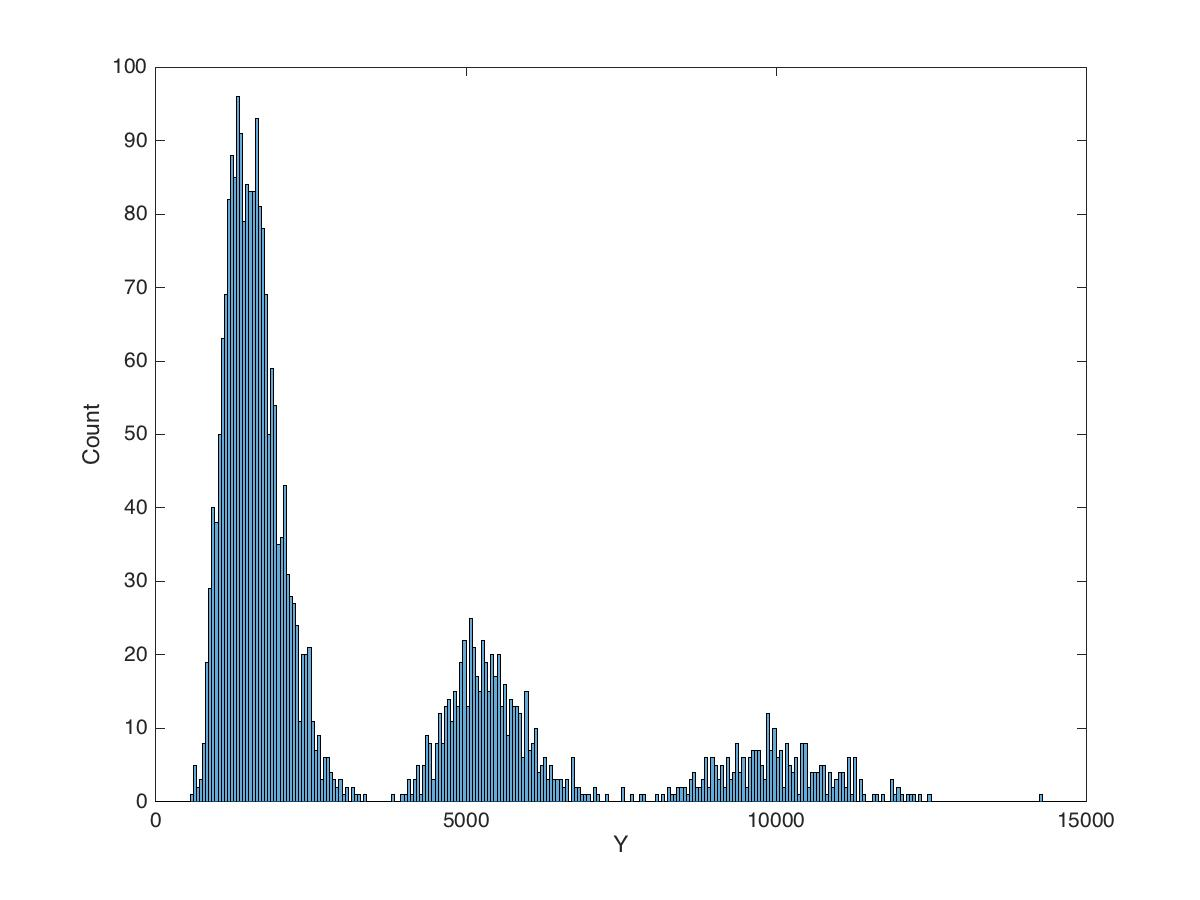
\includegraphics[width=2.7in]{figures/histogram.jpg} \label{fig:histogram}}
\hfill
\subfigure[Feature 2 can help us to separate the data. Green data points are misclassified data. The separation is at $x=0.42$.]{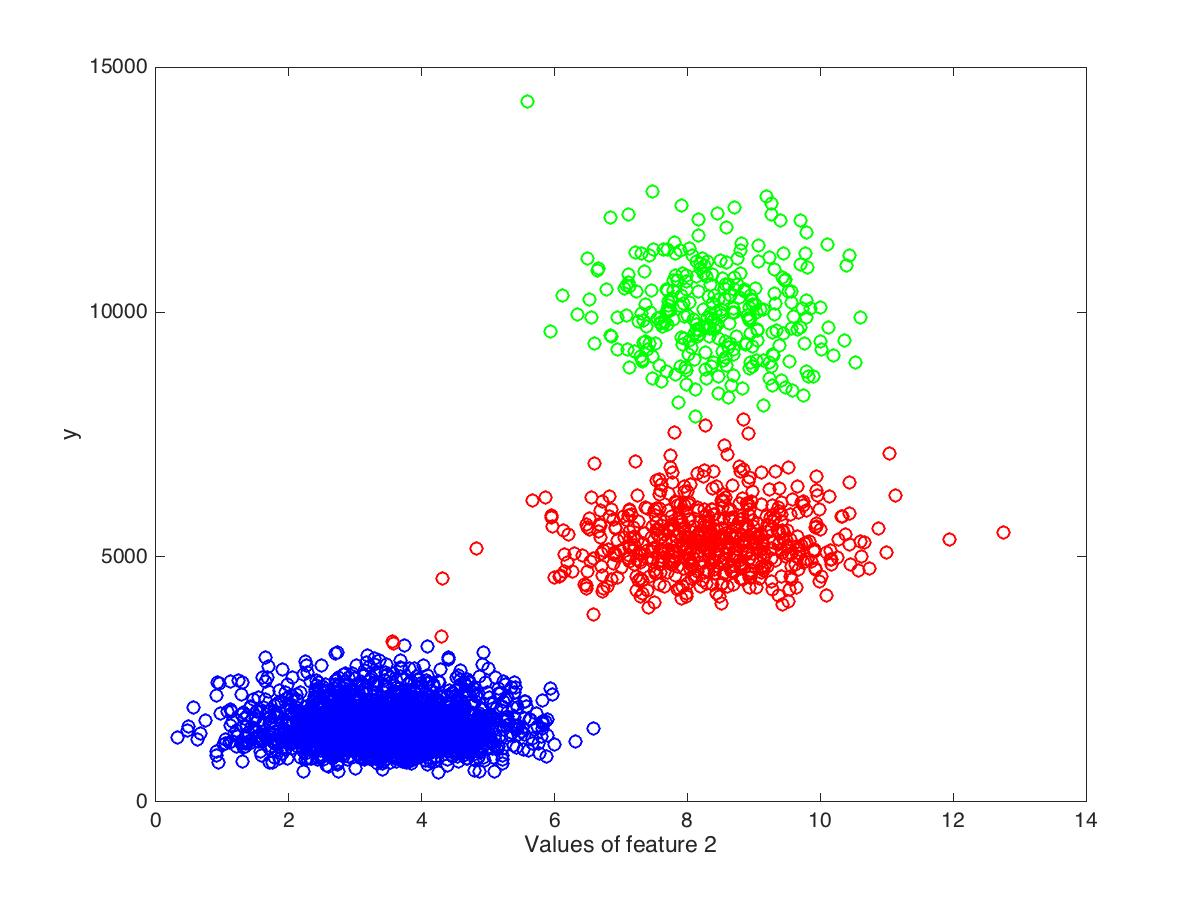
\includegraphics[width=2.7in]{figures/feature2.jpg}\label{fig:feature2}}
\hfill
\subfigure[Feature 16 can help us to separate the data. Green data points are misclassified data. The separation is at $x=1.17$.]{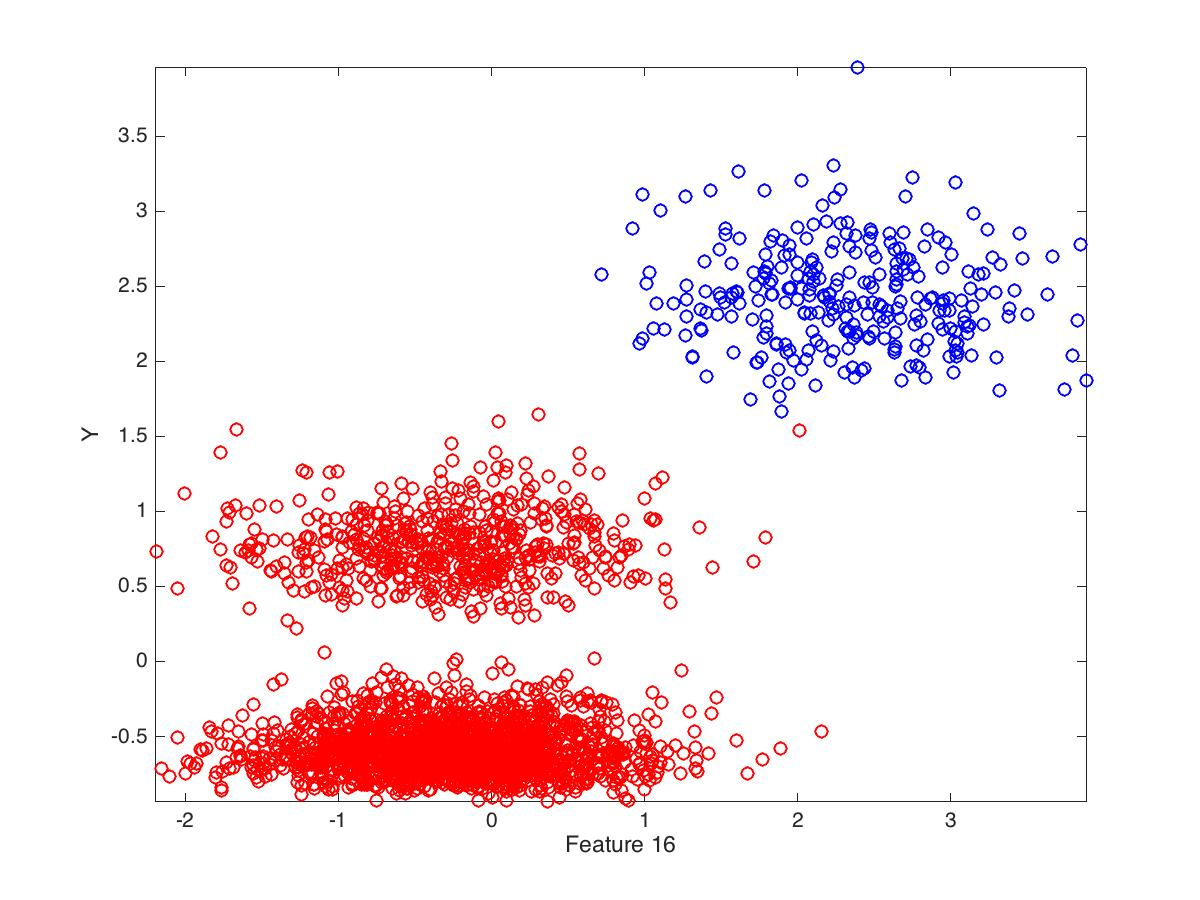
\includegraphics[width=2.7in]{figures/feature16.jpg}\label{fig:feature16}}
\hfill
\subfigure[Different degree for the polynomial basis of the cluster 1. We can observe a low variance. The third degree seems the best model to choose.]{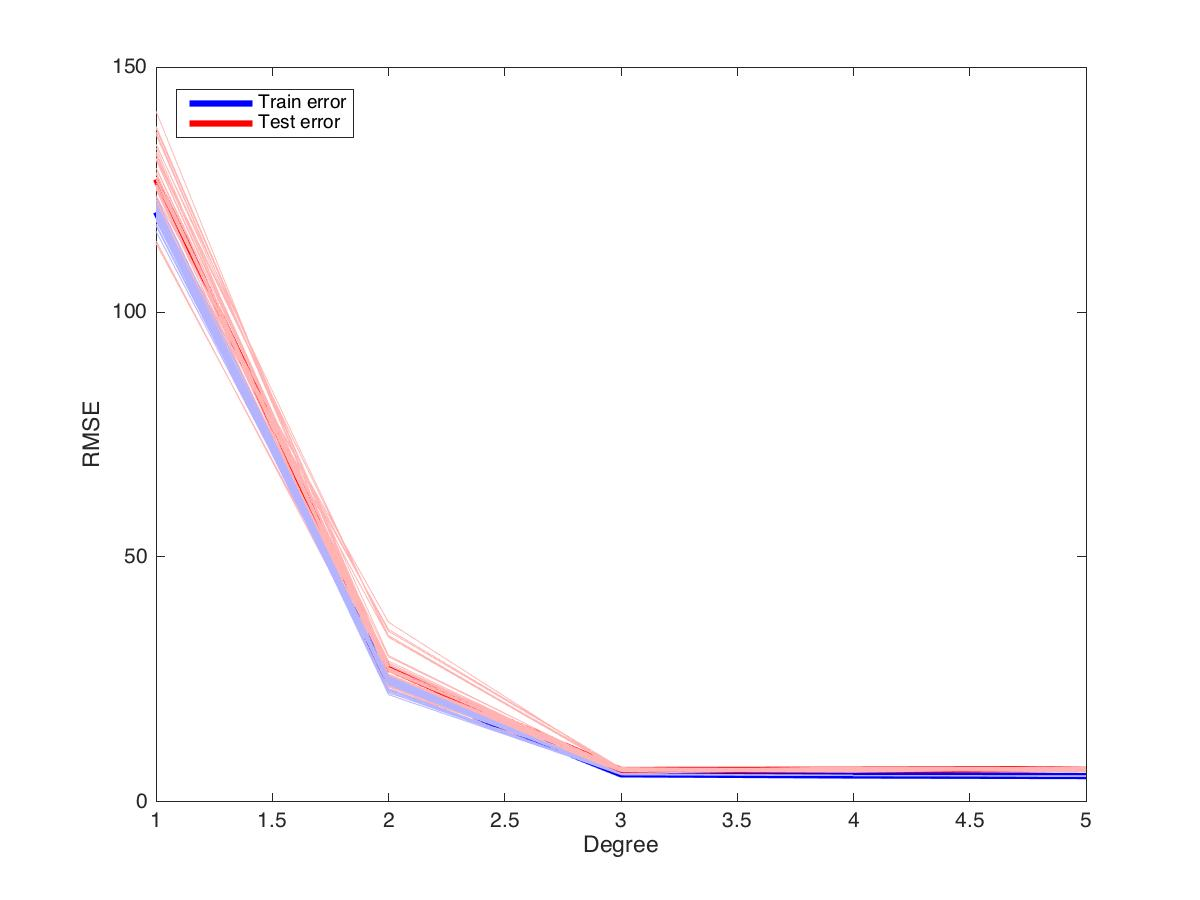
\includegraphics[width=2.7in]{figures/degrees_cls1.jpg}\label{fig:degrees_cls1}}
\hfill
\subfigure[Boxplot of our models, using the RMSE. Each model is represented with a box where we can see their mean and their standard deviation.]{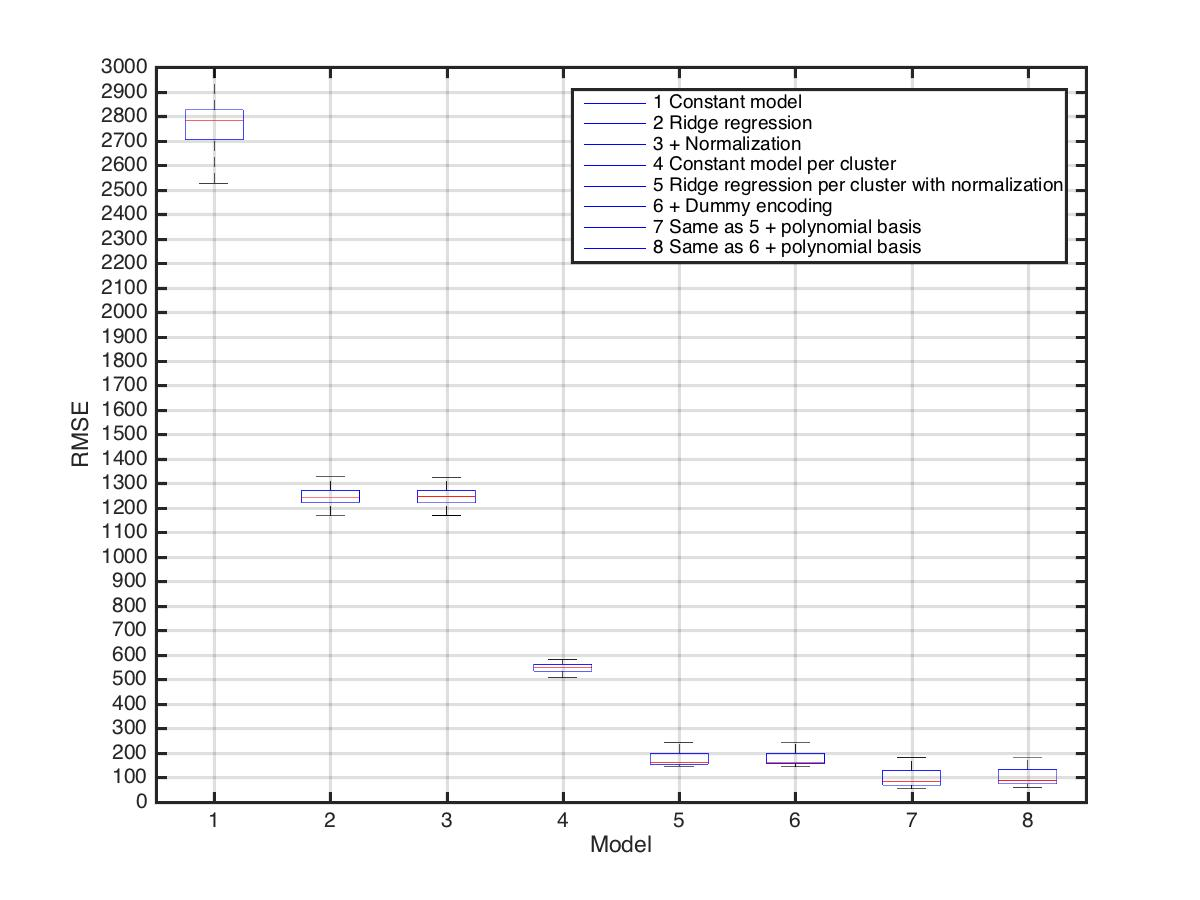
\includegraphics[width=5in]{figures/models.jpg}} \label{fig:models}
\caption{}
\end{figure}

\subsection{Ridge Regression}

Since our matrix is ill-conditioned, using the least squares with normal equation wasn't suitable. Moreover, the results obtained were less good compared to the ridge regression method, and so we will not report those. The method using the least squares with gradient descent was appropriated, but compared to the ridge regression, it was less efficient and was also much slower to tune correctly the learning step. This is the reason why we will not report the results using this method. Therefore, we have so used the ridge regression method, which is suitable because we could lift the eigenvalues in order to avoid ill-conditioned matrix. It is also faster and a little bit more efficient than least squares using gradient descent. Only results obtained with this latter will be reported.

\subsubsection{Evaluation methods}

In order to evaluate our different models, we first have split our data ($\mathbf{X}$) in two sets of $80\%$ and $20\%$, for the training and the test sets. We choose this percentage in order to have still enough data for the training set and also enough to estimate correctly our models on the testing set with a concrete size. We learn only on the training set and then use the test set in order to estimate the error using the \textit{Root Mean Square Error}. Moreover, we have also used k-cross validation (see next section for the values of k) to tune the parameters up like lambda or the different polynomial degrees. We repeated the experiment $30$ times with different seeds in order to split the data in a unique random way for each trial and so try to have an unbiased estimation error. Finally, we made vary the lambda from $10^{-5}$ to $10^{5}$ with $500$ values in-between.

\subsubsection{Model comparison}

The Figure \ref{fig:models} represents the RMSE for each models. The first model used is the constant one, which will allow us to compare improvements with other models. It simply returns the mean of the outputs and doesn't depend on the inputs. Our second model does a ridge regression on the overall data using $10$ fold cross validation, because we have a lot of data, splitting them into $10$ fold seems reasonable. As expected, this is much better than previous model because we take into account the input features. Next model (third) is similar to the second one except that we add normalization on the real inputs (it doesn't make sense to also normalize categorical variables). Normalization is generally a good thing and often a necessity depending on the algorithms used (e.g. gradient descent ones). It improves only slightly but because normalization is a good practice, we have decided to keep it.

At this stage, we want to try to separate our data into clusters. We must be careful because it increases the ill-conditioning ! The fourth model consists of using a constant model but this time separating the data into the three clusters identified during the exploratory data analysis and then computing the mean for each cluster. We can observe a big improvement, justifying our choice to split the data into clusters. The next model (fifth) is about doing a ridge regression per cluster, each one having its own lambda and its own normalization. We also use k-cross validation where the first cluster has a $k_1=10$ because we have a lot of data ($1937$), the second $k_2=6$, because we don't have a lot of data ($563$) and the last $k_3=4$ because we really a small number of data ($273$) and so we have to choose a smaller k. As expected we obtained another big improvement justifying again the choice of splitting the data.

The sixth model consists of using dummy encoding for the categorical variables. As explained in the exploratory data analysis, we use $k-1$ features to represent a $k$ categorical variable. This is a common practice. Unfortunately, we didn't get major improvements. We think that the reason why dummy encoding doesn't help is because we don't have a high bias and so, having more features doesn't help.

The two next models is about using polynomial basis functions for each cluster. Categorical variables aren't concerned, they are just replicated for each degree, because it doesn't make any sense to build polynomial for them. We normalize after the feature transformations, in order to avoid loosing information. We have to be careful about the polynomial degrees to avoid the case where $D > N$ (especially for the cluster two and three, because there are much smaller than the first one). Moreover, if we don't observe significant improvement between degrees, we keep the lowest one. The Figure \ref{fig:degrees_cls1}, shows the case for the first cluster, we can also see that the variance is very low (same observation for the third one, however the second one has higher variance). The seventh model doesn't use dummy encoding and the eighth does.

For the seventh model, the degrees of the polynomial for the clusters are $3,6$ and $3$. When we add higher degrees, we can directly observe overfitting because suddenly the training error decreases to a value near zero and the test errors grows exponentially, so with this manner we know that our degrees are not to high. The eighth model is similar to the seventh one, except that this time it uses dummy encoding and has lower degrees : $3,5$ and $2$, due to the number of input variables ($92$ vs $76$). We can see that these feature transformations significantly improve the prediction accuracy compared to other models. However, dummy encoding doesn't seem to more efficient, and so our final model will be the seventh. 

\subsubsection{Feature transformations}

In hope to minimize the error, we tried different feature transformations. The first try was add polynomial of them self as $X = [X X^2 X^3 ...]$ for which each cluster has its own degree. We made vary the different degrees and also the lambdas in order to keep the lambda which minimizes the test error. We also try feature transformations where the degree is a root, but unfortunately it was worst. We also wanted to try to just pow features with different degrees (without add polynomial of themselves) but we couldn't do it due to a lack of time.

We also thought about removing some uncorrelated features, we tried to remove the most uncorrelated ones and then remove also the second one etc, but unfortunately we didn't get improvements. We think that the reason is that a feature may not be correlated directly with the output however a combination of uncorrelated features might be highly correlated. 

\subsubsection{Summary}

We analyzed a regression data set with different methods and concluded that least squares wasn't a good approach due to the ill-conditioning and the least squares gradient descent was to slow and was less efficient than ridge regression. Moreover, the separation of the data into clusters was essential in order to decrease the prediction accuracy. Unfortunately, dummy encoding didn't help. However using polynomial basis help to decrease the variance. Finally, the variance of cluster 1 and 3 are very low, the one for cluster 2 is a bit higher. We think that we have bias because we use ridge regression but we don't think it is too high because we have seen that adding features helps and at a certain points it wasn't efficient. The best model we have is the seventh one, and we estimate the RMSE of the prediction to be around 97 with a standard deviation of 35. Finally, we think that our model is improvable, however we couldn't try other things in oorder to improve the estimation error, due to a lack of time.

\end{document}
